\documentclass[11pt,preprint, authoryear]{elsarticle}

\usepackage{lmodern}
%%%% My spacing
\usepackage{setspace}
\setstretch{1.2}
\DeclareMathSizes{12}{14}{10}{10}

% Wrap around which gives all figures included the [H] command, or places it "here". This can be tedious to code in Rmarkdown.
\usepackage{float}
\let\origfigure\figure
\let\endorigfigure\endfigure
\renewenvironment{figure}[1][2] {
    \expandafter\origfigure\expandafter[H]
} {
    \endorigfigure
}

\let\origtable\table
\let\endorigtable\endtable
\renewenvironment{table}[1][2] {
    \expandafter\origtable\expandafter[H]
} {
    \endorigtable
}


\usepackage{ifxetex,ifluatex}
\usepackage{fixltx2e} % provides \textsubscript
\ifnum 0\ifxetex 1\fi\ifluatex 1\fi=0 % if pdftex
  \usepackage[T1]{fontenc}
  \usepackage[utf8]{inputenc}
\else % if luatex or xelatex
  \ifxetex
    \usepackage{mathspec}
    \usepackage{xltxtra,xunicode}
  \else
    \usepackage{fontspec}
  \fi
  \defaultfontfeatures{Mapping=tex-text,Scale=MatchLowercase}
  \newcommand{\euro}{€}
\fi

\usepackage{amssymb, amsmath, amsthm, amsfonts}

\def\bibsection{\section*{References}} %%% Make "References" appear before bibliography


\usepackage[round]{natbib}

\usepackage{longtable}
\usepackage[margin=2.3cm,bottom=2cm,top=2.5cm, includefoot]{geometry}
\usepackage{fancyhdr}
\usepackage[bottom, hang, flushmargin]{footmisc}
\usepackage{graphicx}
\numberwithin{equation}{section}
\numberwithin{figure}{section}
\numberwithin{table}{section}
\setlength{\parindent}{0cm}
\setlength{\parskip}{1.3ex plus 0.5ex minus 0.3ex}
\usepackage{textcomp}
\renewcommand{\headrulewidth}{0.2pt}
\renewcommand{\footrulewidth}{0.3pt}

\usepackage{array}
\newcolumntype{x}[1]{>{\centering\arraybackslash\hspace{0pt}}p{#1}}

%%%%  Remove the "preprint submitted to" part. Don't worry about this either, it just looks better without it:
\makeatletter
\def\ps@pprintTitle{%
  \let\@oddhead\@empty
  \let\@evenhead\@empty
  \let\@oddfoot\@empty
  \let\@evenfoot\@oddfoot
}
\makeatother

 \def\tightlist{} % This allows for subbullets!

\usepackage{hyperref}
\hypersetup{breaklinks=true,
            bookmarks=true,
            colorlinks=true,
            citecolor=blue,
            urlcolor=blue,
            linkcolor=blue,
            pdfborder={0 0 0}}


% The following packages allow huxtable to work:
\usepackage{siunitx}
\usepackage{multirow}
\usepackage{hhline}
\usepackage{calc}
\usepackage{tabularx}
\usepackage{booktabs}
\usepackage{caption}


\newenvironment{columns}[1][]{}{}

\newenvironment{column}[1]{\begin{minipage}{#1}\ignorespaces}{%
\end{minipage}
\ifhmode\unskip\fi
\aftergroup\useignorespacesandallpars}

\def\useignorespacesandallpars#1\ignorespaces\fi{%
#1\fi\ignorespacesandallpars}

\makeatletter
\def\ignorespacesandallpars{%
  \@ifnextchar\par
    {\expandafter\ignorespacesandallpars\@gobble}%
    {}%
}
\makeatother

\newlength{\cslhangindent}
\setlength{\cslhangindent}{1.5em}
\newenvironment{CSLReferences}%
  {\setlength{\parindent}{0pt}%
  \everypar{\setlength{\hangindent}{\cslhangindent}}\ignorespaces}%
  {\par}


\urlstyle{same}  % don't use monospace font for urls
\setlength{\parindent}{0pt}
\setlength{\parskip}{6pt plus 2pt minus 1pt}
\setlength{\emergencystretch}{3em}  % prevent overfull lines
\setcounter{secnumdepth}{5}

%%% Use protect on footnotes to avoid problems with footnotes in titles
\let\rmarkdownfootnote\footnote%
\def\footnote{\protect\rmarkdownfootnote}
\IfFileExists{upquote.sty}{\usepackage{upquote}}{}

%%% Include extra packages specified by user

%%% Hard setting column skips for reports - this ensures greater consistency and control over the length settings in the document.
%% page layout
%% paragraphs
\setlength{\baselineskip}{12pt plus 0pt minus 0pt}
\setlength{\parskip}{12pt plus 0pt minus 0pt}
\setlength{\parindent}{0pt plus 0pt minus 0pt}
%% floats
\setlength{\floatsep}{12pt plus 0 pt minus 0pt}
\setlength{\textfloatsep}{20pt plus 0pt minus 0pt}
\setlength{\intextsep}{14pt plus 0pt minus 0pt}
\setlength{\dbltextfloatsep}{20pt plus 0pt minus 0pt}
\setlength{\dblfloatsep}{14pt plus 0pt minus 0pt}
%% maths
\setlength{\abovedisplayskip}{12pt plus 0pt minus 0pt}
\setlength{\belowdisplayskip}{12pt plus 0pt minus 0pt}
%% lists
\setlength{\topsep}{10pt plus 0pt minus 0pt}
\setlength{\partopsep}{3pt plus 0pt minus 0pt}
\setlength{\itemsep}{5pt plus 0pt minus 0pt}
\setlength{\labelsep}{8mm plus 0mm minus 0mm}
\setlength{\parsep}{\the\parskip}
\setlength{\listparindent}{\the\parindent}
%% verbatim
\setlength{\fboxsep}{5pt plus 0pt minus 0pt}



\begin{document}



\begin{frontmatter}  %

\title{Second Semester Notes : Financial Econometrics}

% Set to FALSE if wanting to remove title (for submission)




\author[Add1]{Precious Nhamo\footnote{\textbf{Contributions:}
  \newline \emph{The authors would like to thank no institution for
  money donated to this project. Thank you sincerely.}}}
\ead{pnhamoo@gmail.com}





\address[Add1]{Stellenbosch University, Stellenbosch, South Africa}

\cortext[cor]{Corresponding author: Precious Nhamo\footnote{\textbf{Contributions:}
  \newline \emph{The authors would like to thank no institution for
  money donated to this project. Thank you sincerely.}}}

\begin{abstract}
\small{
In this report I provide an overview of the performance of a South
African equity fund, ABC Fund, relative to its industry peers and the
Capped SWIX benchmark. I focus on rolling three year beta estimates,
relative performance visualisations and the interaction between cross
sectional return dispersion and the fund's performance. The objective is
to help a non quantitative portfolio manager communicate where his fund
offers something different to pure market beta and how this difference
links to periods of high dispersion.
}
\end{abstract}

\vspace{1cm}


\begin{keyword}
\footnotesize{
Multivariate GARCH \sep Kalman Filter \sep Copula \\
\vspace{0.3cm}
}
\footnotesize{
\textit{JEL classification} L250 \sep L100
}
\end{keyword}



\vspace{0.5cm}

\end{frontmatter}



%________________________
% Header and Footers
%%%%%%%%%%%%%%%%%%%%%%%%%%%%%%%%%
\pagestyle{fancy}
\chead{}
\rhead{}
\lfoot{}
\rfoot{\footnotesize Page \thepage}
\lhead{}
%\rfoot{\footnotesize Page \thepage } % "e.g. Page 2"
\cfoot{}

%\setlength\headheight{30pt}
%%%%%%%%%%%%%%%%%%%%%%%%%%%%%%%%%
%________________________

\headsep 35pt % So that header does not go over title




\newpage

\section{Data Preparation}\label{data-preparation}

\section{Rolling Beta Analysis}\label{rolling-beta-analysis}

\pandocbounded{
\includegraphics[keepaspectratio]{Q1_files/figure-latex/rolling-beta-1.pdf}}

\pandocbounded{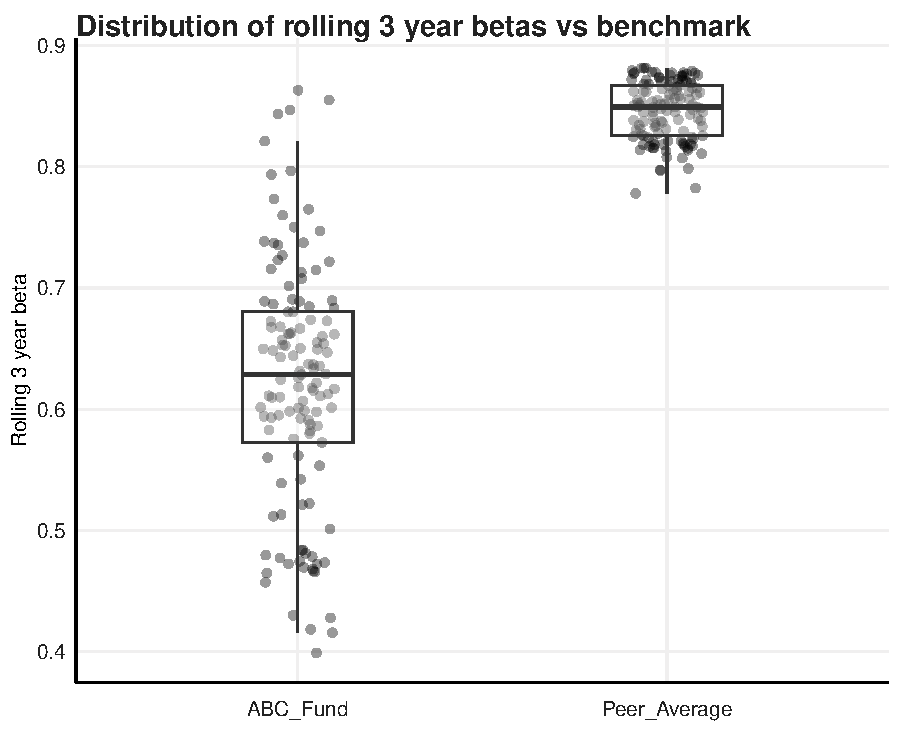
\includegraphics[keepaspectratio]{Q1_files/figure-latex/boxplot-beta-1.pdf}}

\section{Performance Analysis}\label{performance-analysis}

\begin{verbatim}
##                 Benchmark ABC_Fund Peer_Average
## Observations     160.0000 160.0000     160.0000
## NAs                0.0000   0.0000       0.0000
## Minimum           -0.1669  -0.0715      -0.1486
## Quartile 1        -0.0150  -0.0040      -0.0130
## Median             0.0141   0.0123       0.0127
## Arithmetic Mean    0.0099   0.0117       0.0084
## Geometric Mean     0.0091   0.0112       0.0079
## Quartile 3         0.0321   0.0290       0.0268
## Maximum            0.1418   0.1509       0.1303
## SE Mean            0.0030   0.0024       0.0026
## LCL Mean (0.95)    0.0039   0.0069       0.0033
## UCL Mean (0.95)    0.0158   0.0165       0.0135
## Variance           0.0014   0.0009       0.0011
## Stdev              0.0379   0.0308       0.0329
## Skewness          -0.4396   0.2528      -0.4085
## Kurtosis           2.8386   2.0787       3.3731
\end{verbatim}

\begin{verbatim}
##                       Benchmark ABC_Fund Peer_Average
## Last 3 month Average     0.0396   0.0304       0.0307
## Last 6 month Average     0.0322   0.0278       0.0282
## Last 12 month Average    0.0234   0.0163       0.0174
## Last 36 month Average    0.0161   0.0118       0.0134
## Last 60 month Average    0.0162   0.0140       0.0139
## Last 3 month Std Dev     0.0239   0.0139       0.0132
## Last 6 month Std Dev     0.0174   0.0105       0.0098
## Last 12 month Std Dev    0.0213   0.0170       0.0149
## Last 36 month Std Dev    0.0362   0.0228       0.0290
## Last 60 month Std Dev    0.0365   0.0256       0.0302
\end{verbatim}

\begin{verbatim}
##                     ABC_Fund to Benchmark Peer_Average to Benchmark
## Alpha                              0.0056                    0.0001
## Beta                               0.6160                    0.8450
## Alpha Robust                       0.0059                    0.0002
## Beta Robust                        0.5991                    0.8453
## Beta+                              0.6527                    0.8610
## Beta-                              0.4864                    0.8684
## Beta+ Robust                       0.6346                    0.8593
## Beta- Robust                       0.4871                    0.8691
## R-squared                          0.5761                    0.9507
## R-squared Robust                   0.5248                    0.9285
## Annualized Alpha                   0.0693                    0.0010
## Correlation                        0.7590                    0.9750
## Correlation p-value                0.0000                    0.0000
## Tracking Error                     0.0858                    0.0325
## Active Premium                     0.0277                   -0.0167
## Information Ratio                  0.3229                   -0.5128
## Treynor Ratio                      0.2322                    0.1167
\end{verbatim}

\pandocbounded{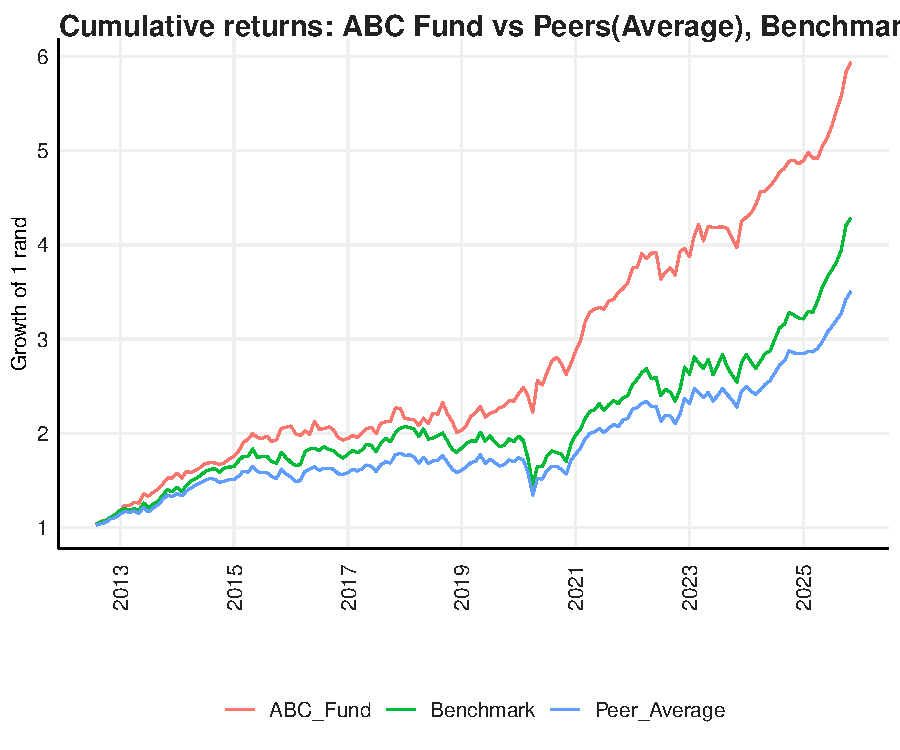
\includegraphics[keepaspectratio]{Q1_files/figure-latex/cumulative-returns-1.pdf}}

\pandocbounded{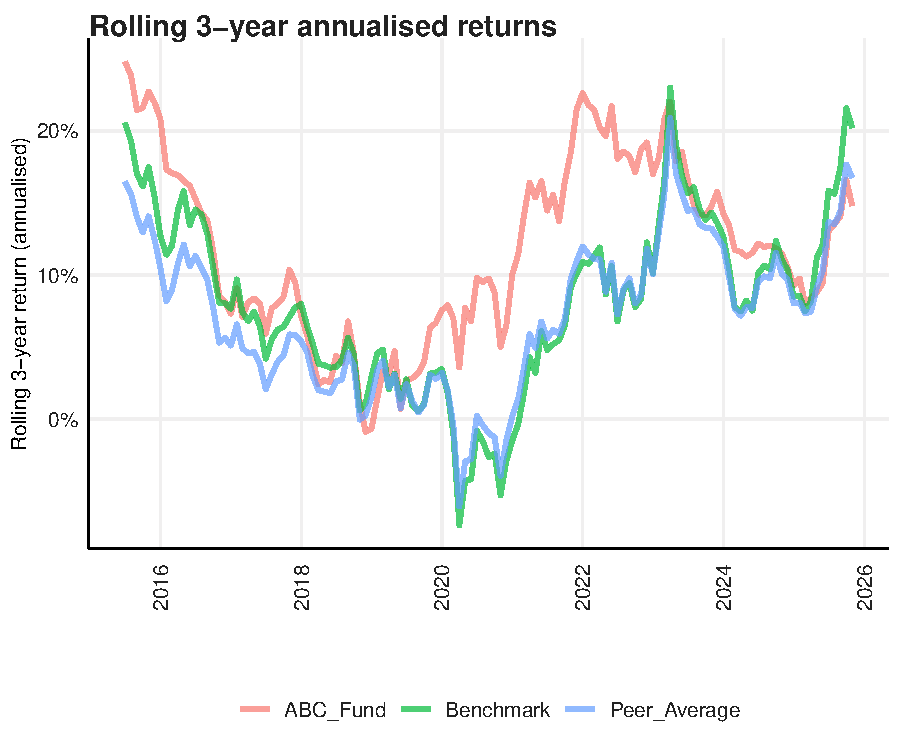
\includegraphics[keepaspectratio]{Q1_files/figure-latex/rolling-returns-1.pdf}}

\pandocbounded{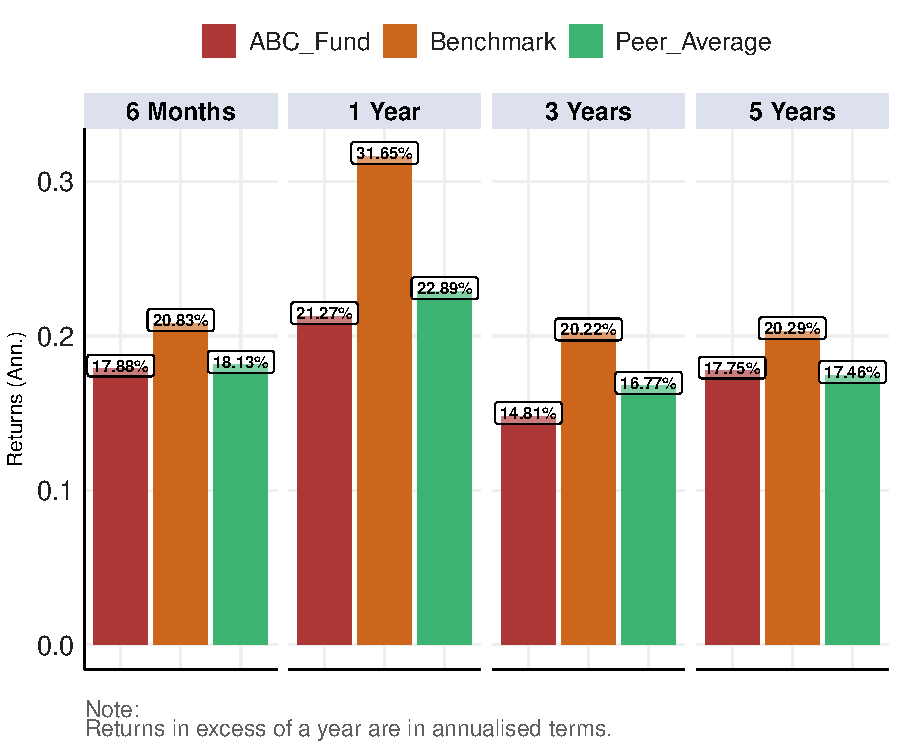
\includegraphics[keepaspectratio]{Q1_files/figure-latex/annualised-returns-1.pdf}}

\pandocbounded{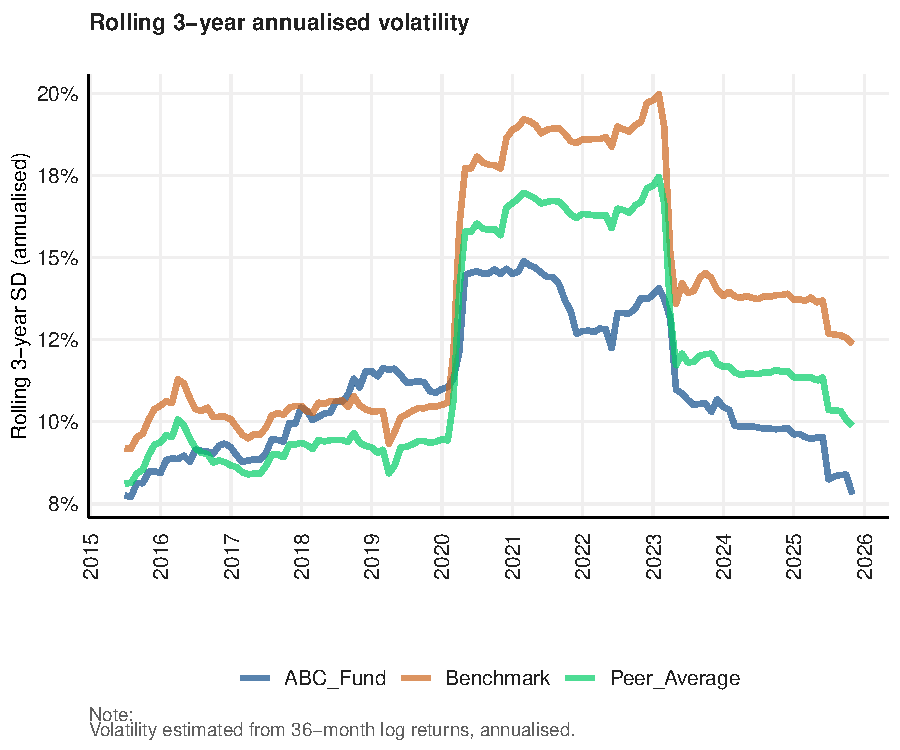
\includegraphics[keepaspectratio]{Q1_files/figure-latex/volatility-1.pdf}}

\bibliography{Tex/ref}





\end{document}
